% !TEX root = ./report.tex
\documentclass[12pt, a4paper]{article}
\usepackage[a4paper, margin=1.0in, foot=.25in]{geometry}
% Detect lualatex
\usepackage{ifluatex}
\ifluatex\else\errmessage{Please use LuaLaTex.}\stop\fi

% ----------------------------
% Fonts
% ----------------------------
\usepackage{luatexja}
\usepackage{luatexja-fontspec}
% English font
\setmainfont[ExternalLocation=fonts/]{linlibertine_re-4.7.5ro.ttf}[
    Ligatures=TeX,
    BoldFont=linlibertine_bd-4.1.5ro.ttf,
    ItalicFont=linlibertine_it-4.2.6ro.ttf
]
% Chinese font
% 思源宋體
\setmainjfont[Scale=0.85,ExternalLocation=fonts/]{NotoSerifTC-Regular.otf}[
    Ligatures=TeX,
    BoldFont=NotoSerifTC-Bold.otf,
    ItalicFont=NotoSerifTC-Regular.otf,
    BoldItalicFont=NotoSerifTC-Regular.otf,
]
% 芫荽體
% \setmainjfont[Scale=0.85,ExternalLocation=./fonts/]{Iansui-Regular.ttf}
% font for code
\newfontfamily{\Iosevka}[Path=./fonts/, Scale=0.86]{iosevka-fixed-ss15-regular.ttf}
\newfontfamily{\IosevkaItalic}[Path=./fonts/, Scale=0.86]{iosevka-fixed-ss15-italic.ttf}
\newfontfamily{\IosevkaBold}[Path=./fonts/, Scale=0.86]{iosevka-fixed-ss15-bold.ttf}

% ----------------------------
% Bibliography
% ----------------------------
\usepackage[backend=biber,maxbibnames=99,sorting=ynt,isbn=false]{biblatex} 
\renewcommand{\cite}{\autocite}
\addbibresource{report.bib}

% ----------------------------
% Code 
% ----------------------------
\usepackage{listings}
\usepackage[dvipsnames]{xcolor} % color
\usepackage[most]{tcolorbox}
\tcbset{on line, 
    boxsep=0pt, left=3pt,right=3pt,top=2pt,bottom=2pt,
    colframe=white,  
    highlight math style={enhanced}
}
% my color
\definecolor{MyRed}{HTML}{FF6666}
\definecolor{MyGreen}{HTML}{00CC00}
\definecolor{MyBlue}{HTML}{3399FF}
\definecolor{MyOrange}{HTML}{FF9933}
\definecolor{MyGreenBG}{HTML}{CCFF99}
\definecolor{MyYellowBG}{HTML}{FFFF99}
\definecolor{MyGreyBG}{HTML}{E6E6E6}

% copy indent from the code
\lstset{keepspaces=true}
\makeatletter
\def\lst@outputspace{{\ifx\lst@bkgcolor\empty\color{white}\else\lst@bkgcolor\fi\lst@visiblespace}}
\makeatother

% make line number of code no be copied
% https://tex.stackexchange.com/a/122270
\usepackage[space=true]{accsupp}    
\newcommand{\noncopynumber}[1]{%
    \BeginAccSupp{method=escape,ActualText={}}%
    #1%
    \EndAccSupp{}%
}

% Python style for highlighting
\newcommand\pythonstyle{\lstset{%
language=Python,%
basicstyle=\Iosevka,%
morekeywords={self,with},% Add keywords here
keywordstyle=\IosevkaBold\color{BlueViolet},%
emph={MyClass,__init__},% Custom highlighting
emphstyle=\IosevkaBold\color{BrickRed},% Custom highlighting style
stringstyle=\color{ForestGreen},%
frame=single,% Any extra options here
showstringspaces=false,%
showspaces=true,%
commentstyle=\IosevkaItalic\color{Gray},%
morecomment=[l][\IosevkaItalic\color{Gray}]{\#},%
numbers=left,%
stepnumber=1,%
literate={-}{-}1,%
columns=fullflexible,%
numberstyle=\footnotesize\noncopynumber,%
mathescape=true,% show math equation, e.g., $x = \sqrt{2}$
}}
% remove space char
\makeatletter
\def\lst@visiblespace{ }
\makeatother
% Python for inline
\newcommand\pythoninline[1]{%
    {\pythonstyle\lstinline[breaklines=false]{#1}}}
\newcommand\pythoninlinebg[1]{%
\tcbox[colback=MyGreyBG]{{\pythonstyle\lstinline[breaklines=false]{#1}}}%
}
% Python for block
\lstnewenvironment{python}[1][]{%
    \pythonstyle\footnotesize\lstset{#1}%
}{}

% ----------------------------
% links of cite, ref
% ----------------------------
\usepackage{xurl} % url wrap
\usepackage{hyperref}
\hypersetup{
    colorlinks,
    linkcolor=[RGB]{120, 29, 125},
    citecolor=[RGB]{120, 29, 125},
    urlcolor=[RGB]{0, 85, 150}
}

% ----------------------------
% Figure
% ----------------------------
\usepackage{graphicx} % figure
\usepackage{caption}

% ----------------------------
% Misc.
% ----------------------------
\usepackage{placeins} % \FloatBarrier
\usepackage{booktabs} % \toprule, \midrule, \bottomrule
\renewcommand{\figurename}{圖}
\newcommand{\sectionname}{節}
\newcommand{\chaptername}{章}
\renewcommand{\tablename}{表}
\renewcommand{\lstlistingname}{程式碼}
\newcommand{\Figure}[1]{\figurename~#1}
\newcommand{\Table}[1]{\tablename~#1}
\newcommand{\Section}[1]{\sectionname~#1}
\newcommand{\Chapter}[1]{\chaptername~#1}
\newcommand{\Listing}[1]{\lstlistingname~#1}

\title{繁體中文標題}

\author{作者:黃柏瑄\\ 
    \texttt{aben20807@gmail.com}
}

\date{} % skip date

\begin{document}

\maketitle

\section{介紹}\label{sec:first}

這是一個關於 LaTeX 的介紹。測試引用功能 \cite{huang2023securetvm}。

\subsection{第一節的一個小節}\label{sec:first_sub}

這是第一章的一個小節。參見第 \ref{sec:second} 節中的更多細節。

\section{第二節標題}\label{sec:second}

這是第二節的內容。\textcolor{MyRed}{參見}第 \ref{sec:first} 節以獲得\textcolor[HTML]{FF6666}{更多資訊}。

\section{程式碼}\label{sec:code}

使用行內程式碼,\pythoninline{print("Hello")},也可以使用有背景顏色版本\pythoninlinebg{x = 42}。程式碼區塊如下方~\Listing{\ref{list:example}}。

\begin{python}[caption={定義 \protect\pythoninlinebg{main} 函式。},label=list:example,escapechar=|]
def main():
    x = 42
    print(f"Hello {x}")

if __name__ == "__main__":
    main()
\end{python}

\section{圖片}

參考~\Figure{\ref{fig:A}} 和~\Figure{\ref{fig:B}}。

\begin{table}[t]
    \centering
    \begin{minipage}[t]{.48\linewidth}
        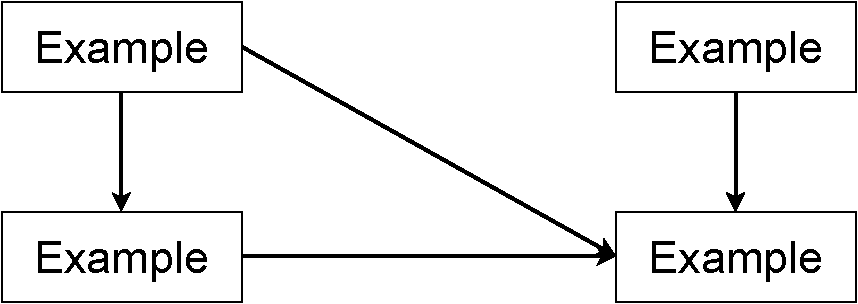
\includegraphics[width=\linewidth]{figures/paper-example.pdf}
        \captionof{figure}{第一張圖。}
        \label{fig:A}
    \end{minipage}
    \qquad
    \begin{minipage}[t]{.44\linewidth}
        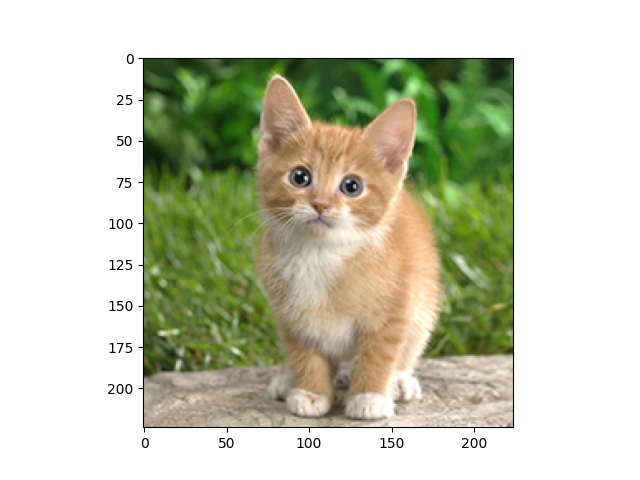
\includegraphics[width=\linewidth]{figures/cat.png}
        \captionof{figure}{第二張圖。}
        \label{fig:B}
    \end{minipage}
\end{table}

\section{表格}

參考~\Table{\ref{tab:example}}。

\begin{table}[t]
    \centering
    \caption{表格說明。}\label{tab:example}
    \begin{tabular}{lll}
    \toprule
    \textbf{Category} & \textbf{Work} & \textbf{Tags} \\
    \midrule
        Open     &   Title A   &   A, B, C   \\
        Open     &   Title B   &  B, D    \\
        Close     &   Title C   &  A, B, D    \\
        Close     &   ``Title D''   &  E \pythoninlinebg{TestClass}   \\
    \bottomrule
    \end{tabular}
\end{table}

\FloatBarrier
\renewcommand*{\bibfont}{\small}
\printbibliography[
    heading=bibintoc,
    title={參考文獻}
]

\end{document}